\documentclass[a4paper]{article}
\usepackage{tikz}
\usepackage{geometry}
\usepackage{graphicx}
\usepackage{natbib}
\usepackage{amsmath}
\usepackage{amssymb}
\usepackage{amsthm}
\usepackage{paralist}
\usepackage{epstopdf}
\usepackage{tabularx}
\usepackage{longtable}
\usepackage{multirow}
\usepackage{multicol}
\usepackage[hidelinks]{hyperref}
\usepackage{fancyvrb}
\usepackage{algorithm}
\usepackage{algorithmic}
\usepackage{float}
\usepackage{paralist}
%\usepackage[svgname]{xcolor}
\usepackage{enumerate}
\usepackage{array}
\usepackage{times}
\usepackage{url}
\usepackage{fancyhdr}
\usepackage{comment}
\usepackage{environ}
\usepackage{times}
\usepackage{textcomp}
\usepackage{caption}
\usepackage{bbm}


\urlstyle{rm}

\setlength\parindent{0pt} % Removes all indentation from paragraphs
\theoremstyle{definition}
\newtheorem{definition}{Definition}[]
\newtheorem{conjecture}{Conjecture}[]
\newtheorem{example}{Example}[]
\newtheorem{theorem}{Theorem}[]
\newtheorem{lemma}{Lemma}
\newtheorem{proposition}{Proposition}
\newtheorem{corollary}{Corollary}

\floatname{algorithm}{Procedure}
\renewcommand{\algorithmicrequire}{\textbf{Input:}}
\renewcommand{\algorithmicensure}{\textbf{Output:}}
\newcommand{\abs}[1]{\lvert#1\rvert}
\newcommand{\norm}[1]{\lVert#1\rVert}
\newcommand{\RR}{\mathbb{R}}
\newcommand{\CC}{\mathbb{C}}
\newcommand{\Nat}{\mathbb{N}}
\newcommand{\br}[1]{\{#1\}}
\DeclareMathOperator*{\argmin}{arg\,min}
\DeclareMathOperator*{\argmax}{arg\,max}
\renewcommand{\qedsymbol}{$\blacksquare$}

\definecolor{dkgreen}{rgb}{0,0.6,0}
\definecolor{gray}{rgb}{0.5,0.5,0.5}
\definecolor{mauve}{rgb}{0.58,0,0.82}

\definecolor{C0}{HTML}{1F77B4}
\definecolor{C1}{HTML}{FF7F0E}
\definecolor{C2}{HTML}{2ca02c}
\definecolor{C3}{HTML}{d62728}
\definecolor{C4}{HTML}{9467bd}
\definecolor{C5}{HTML}{8c564b}
\definecolor{C6}{HTML}{e377c2}
\definecolor{C7}{HTML}{7F7F7F}
\definecolor{C8}{HTML}{bcbd22}
\definecolor{C9}{HTML}{17BECF}

\newcommand{\Var}{\mathrm{Var}}
\newcommand{\Cov}{\mathrm{Cov}}
\newcommand{\sgn}{\mathrm{sgn}}

\newcommand{\vc}[1]{\boldsymbol{#1}}
\newcommand{\xv}{\vc{x}}
\newcommand{\Sigmav}{\vc{\Sigma}}
\newcommand{\alphav}{\vc{\alpha}}
\newcommand{\muv}{\vc{\mu}}

\newcommand{\red}[1]{\textcolor{red}{#1}}

\def\x{\mathbf x}
\def\y{\mathbf y}
\def\w{\mathbf w}
\def\v{\mathbf v}
\def\E{\mathbb E}
\def\R{\mathbb R}
\def\V{\mathbb V}
\def\ind{\mathbbm 1}

% TO SHOW SOLUTIONS, include following (else comment out):
\newenvironment{soln}{
    \leavevmode\color{blue}\ignorespaces
}{}


\hypersetup{
%    colorlinks,
    linkcolor={red!50!black},
    citecolor={blue!50!black},
    urlcolor={blue!80!black}
}

\geometry{
  top=1in,            % <-- you want to adjust this
  inner=1in,
  outer=1in,
  bottom=1in,
  headheight=3em,       % <-- and this
  headsep=2em,          % <-- and this
  footskip=3em,
}


\pagestyle{fancyplain}
\lhead{\fancyplain{}{Homework 8}}
\rhead{\fancyplain{}{CS 760 Machine Learning}}
\cfoot{\thepage}

\title{\textsc{Homework 8}} % Title

%%% NOTE:  Replace 'NAME HERE' etc., and delete any "\red{}" wrappers (so it won't show up as red)

\author{
\red{$AKASH SHARMA$} \\
\red{$9081731771$}\\
} 

\date{}

\begin{document}

\maketitle 


\textbf{Instructions:} 
Although this is a programming homework, you only need to hand in a pdf answer file.
There is no need to submit the latex source or any code.
You can choose any programming language, as long as you implement the algorithm from scratch.

Use this latex file as a template to develop your homework.
Submit your homework on time as a single pdf file to Canvas.
Please check Piazza for updates about the homework.


\section{Directed Graphical Model [20 points]}
Consider the directed graphical model (aka Bayesian network) in Figure~\ref{fig:bn}.
\begin{figure}[H]
        \centering
                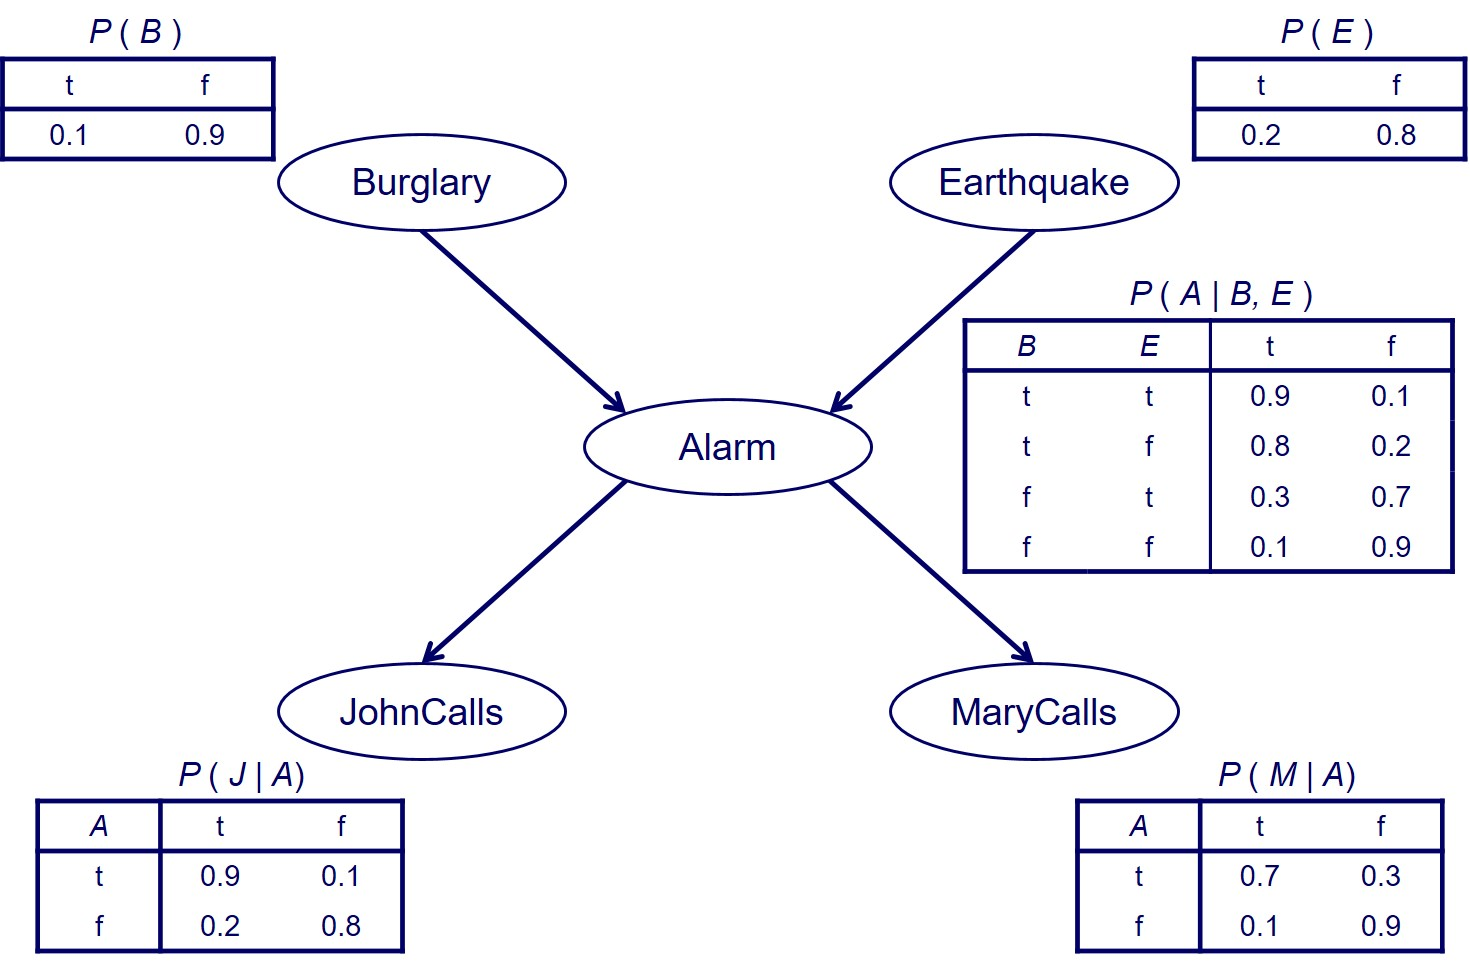
\includegraphics[width=0.8\textwidth]{BN.jpg}
        \caption{A Bayesian Network example.}
        \label{fig:bn}
\end{figure}
Compute $P(B=t \mid E=f,J=t,M=t)$ and $P(B=t \mid E=t,J=t,M=t)$.
These are the conditional probabilities of a burglar in your house (yikes!) when both of your neighbors John and Mary call you and say they hear an alarm in your house, but without or with an earthquake also going on in that area (what a busy day), respectively.


\begin{soln}
1. $P(B=t \mid E=f,J=t,M=t) = \frac{P(B=t,E=f,J=t,M=t)}{P(E=f,J=t,M=t)}$ \\ \\
The numerator, 
$P(B=t,E=f,J=t,M=t)$ can be written as,\\
$=P(B=t,E=f,J=t,M=t,A=t) + P(B=t,E=f,J=t,M=t,A=f)$ \\
$= P(B=t) \times P(E=f) [\;P(M=t \mid A=t) \times P(J=t \mid A=t) \times P(A=t \mid B=t,E=f) + \\
P(J=t \mid A=f) \times P(M=t \mid A=f) \times P(A=f \mid B=t,E=f)\;] \\$
$=0.1 \times 0.8 \times 0.2 \times 0.1 \times 0.2 + 0.1 \times 0.8 \times 0.9 \times 0.7 \times 0.8$
$=0.04064$ \\ \\
Similarly, the denominator $P(E=f,J=t,M=t)$,\\
$=P(E=f,J=t,M=t,A=t,B=t) + P(E=f,J=t,M=t,A=t,B=f) + \\P(E=f,J=t,M=t,A=f,B=t) + P(E=f,J=t,M=t,A=f,B=f)$ \\
$=P(E=f) \times $   $[\;  
P(B=t) \times P(J=t \mid A=f) \times P(M=t \mid A=f) \times P(A=f \mid E=f,B=t) + \\
P(B=f) \times P(J=t \mid A=t) \times P(M=t \mid A=t) \times P(A=t \mid E=f,B=f) + \\
P(B=t) \times P(J=t \mid A=t) \times P(M=t \mid A=t) \times P(A=t \mid E=f,B=t) + \\
P(B=f) \times P(J=t \mid A=f) \times P(M=t \mid A=f) \times P(A=f \mid E=f,B=f) \;]$ \\
$= 0.8 \times 0.1 \times 0.9 \times 0.7 \times 0.8  +  0.8 \times 0.9 \times 0.9 \times 0.7 \times 0.1 +
0.8 \times 0.1 \times 0.2 \times 0.1 \times 0.2 + 0.8 \times 0.9 \times 0.2 \times 0.1 \times 0.9 $ \\
$= 0.09896$ \\
So, dividing the numerator and denominator calculated above, we get,
\\$P(B=t \mid E=f,J=t,M=t) = \frac{0.04064}{0.09896} = 0.41067$ \\ \\


2. $P(B=t \mid E=t,J=t,M=t) = \frac{P(B=t,E=t,J=t,M=t)}{P(E=t,J=t,M=t)}$ \\ 
The numerator, $P(B=t,E=t,J=t,M=t)\\
=P(B=t,E=t,J=t,M=t,A=t) + P(B=t,E=t,J=t,M=t,A=f)$ \\
$= P(B=t) \times P(E=t) [\;P(J=t \mid A=t) \times P(M=t \mid A=t) \times P(A=t \mid B=t,E=t) + \\
P(J=t \mid A=f) \times P(M=t \mid A=f) \times P(A=f \mid B=t,E=t)\;] \\$
$=0.1 \times 0.2 \times 0.9 \times 0.7 \times 0.9 + 0.1 \times 0.2 \times 0.2 \times 0.1 \times 0.1$
$=0.01138$ \\ \\
The denominator, $P(E=t,J=t,M=t)\\
=P(E=t,J=t,M=t,A=t,B=t) + P(E=t,J=t,M=t,A=t,B=f) + P(E=t,J=t,M=t,A=f,B=t) + P(E=t,J=t,M=t,A=f,B=f)$ \\
$=P(E=t) \times $   $[\;  
P(B=t) \times P(J=t \mid A=t) \times P(M=t \mid A=t) \times P(A=t \mid E=t,B=t) + \\
P(B=f) \times P(J=t \mid A=t) \times P(M=t \mid A=t) \times P(A=t \mid E=t,B=f) + \\
P(B=t) \times P(J=t \mid A=f) \times P(M=t \mid A=f) \times P(A=f \mid E=t,B=t) + \\
P(B=f) \times P(J=t \mid A=f) \times P(M=t \mid A=f) \times P(A=f \mid E=t,B=f) \;]$ \\
$= 0.2 \times 0.1 \times 0.9 \times 0.7 \times 0.9 + 0.2 \times 0.9 \times 0.9 \times 0.7 \times 0.3 +
0.2 \times 0.1 \times 0.2 \times 0.1 \times 0.1 + 0.2 \times 0.9 \times 0.2 \times 0.1 \times 0.7 $ \\
$= 0.04792$ \\
So, dividing the numerator and denominator calculated above, we get,\\
$ P(B=t \mid E=t,J=t,M=t) = \frac{0.01138}{0.04792} = 0.23747$ \\ \\


\end{soln}



\section{Chow-Liu Algorithm [20 pts]}
Suppose we wish to construct a directed graphical model for 3 features $X$, $Y$, and $Z$ using the Chow-Liu algorithm. We are given data from 100 independent experiments where each feature is binary and takes value $T$ or $F$. Below is a table summarizing the observations of the experiment:

\begin{table}[H]
        \centering
                \begin{tabular}{cccc}
                           $X$ & $Y$ & $Z$ & Count \\
                                \hline
                                T & T & T & 36 \\
                                \hline
                                T & T & F & 4 \\
                                \hline
                                T & F & T & 2 \\
                                \hline
                                T & F & F & 8 \\
                                \hline
                                F & T & T & 9 \\
                                \hline
                                F & T & F & 1 \\
                                \hline
                                F & F & T & 8 \\
                                \hline
                                F & F & F & 32 \\
                                \hline
                \end{tabular}
\end{table}

\begin{enumerate}
\item Compute the mutual information $I(X, Y)$ based on the frequencies observed in the data.
\begin{soln} \\ \\
$I(X, Y) = \sum_{ x \in \{t,f \} } \sum_{ y \in \{t,f \} } \; P(x,y) \times \log_2{\frac{P(x,y)}{P(x)\times P(y)}}$ \\ \\
$ = 
0.4 \times \log_2{\frac{0.4}{0.5 \times 0.5}} \; +
0.1 \times \log_2{\frac{0.1}{0.5 \times 0.5}} \; +
0.4 \times \log_2{\frac{0.4}{0.5 \times 0.5}} \; +
0.1 \times \log_2{\frac{0.1}{0.5 \times 0.5}}$ \\ \\
So, solving the above, $I(X, Y) = 0.27807$
\end{soln}


\item Compute the mutual information $I(X, Z)$ based on the frequencies observed in the data.
\begin{soln} \\ \\
$I(X, Z) = \sum_{ x \in \{t,f \} } \sum_{ z \in \{t,f \} } \; P(x,z) \times \log_2{\frac{P(x,z)}{P(x)\times P(z)}}$ \\ \\
$ = 
0.12 \times \log_2{\frac{0.12}{0.5 \times 0.45}} \; +
0.38 \times \log_2{\frac{0.38}{0.5 \times 0.55}} \; +
0.17 \times \log_2{\frac{0.17}{0.5 \times 0.55}} \; +
0.33 \times \log_2{\frac{0.33}{0.5 \times 0.45}}$ \\ \\
So, solving the above, $ I(X, Z) = 0.13284$
\end{soln}



\item Compute the mutual information $I(Z, Y)$ based on the frequencies observed in the data.
\begin{soln} \\ \\
$I(Y, Z) = \sum_{ y \in \{t,f \} } \sum_{ z \in \{t,f \} } \; P(y,z) \times \log_2{\frac{P(y,z)}{P(y)\times P(z)}}$ \\ \\
$ = 
0.45 \times \log_2{\frac{0.45}{0.5 \times 0.55}} \; +
0.05 \times \log_2{\frac{0.05}{0.5 \times 0.45}} \; +
0.4 \times \log_2{\frac{0.4}{0.5 \times 0.45}} \; +
0.1 \times \log_2{\frac{0.1}{0.5 \times 0.55}}$ \\ \\
So, solving the above, $ I(Y, Z) = 0.39731$
\end{soln}



\item Which undirected edges will be selected by the Chow-Liu algorithm as the maximum spanning tree?
\begin{soln}
\\Chow-Liu algorithm will choose edges X--Y and Y--Z for the maximum spanning tree.
\end{soln}



\item Root your tree at node $X$, assign directions to the selected edges.
\begin{soln}
\\ \\ Directions assigned are: 
$ X \rightarrow Y \rightarrow Z $
\end{soln}

\end{enumerate}


\section{Kernel SVM [20 points]}
Consider the following kernel function defined over $z,z'\in Z$:
\begin{align*}
k(z,z') =
\begin{cases}
1 & \text{~if~} z=z', \\
0 & \text{~otherwise.}
\end{cases}
\end{align*}
\begin{enumerate}
\item Prove that for any integer $m>0$, any $z_1, \ldots, z_m \in Z$, the $m \times m$ kernel matrix $K=[K_{ij}]$ is positive semi-definite, where $K_{ij}=k(z_i, z_j)$ for $i,j=1\ldots m$.
Hint: An $m\times m$ matrix $K$ is positive semi-definite if $\forall v \in \R^m, v^\top K v \ge 0$.

\begin{soln}

$$
K= \begin{bmatrix}
k(z_1,z_1)&...&k(z_1,z_m)\\
.&...&.\\
.&...&.\\
k(z_m,z_1)&...&k(z_m,z_m)\\
\end{bmatrix}
$$

$K_{ij}$ = 1, where $i=j$, and $K_{ij}$ = 0,  where $i \neq j.$, that is all the diagonal entries will be 1 and the matrix will be symmetric.
We need to prove that $\forall v \in \R^m, v^\top K v \ge 0$ for K to be a positive semi-definite matrix. 

So,
$$
K = \begin{bmatrix}
1&...&k(z_1,z_m)\\
.&...&.\\
.&...&.\\
k(z_m,z_1)&...&1\\
\end{bmatrix}
$$
Now $\forall v \in \R^m, v^\top K v $ = $ \begin{bmatrix}v_1&v_2 &... &v_m \end{bmatrix}$$\begin{bmatrix}
1&...&k(z_1,z_m)\\
.&...&.\\
.&...&.\\
k(z_m,z_1)&...&1\\
\end{bmatrix}$
$ \begin{bmatrix}v_1\\v_2 \\ .\\.\\ v_m \end{bmatrix}$

$ = v_1^2 + v_2^2 +...+ v_m^2 + 2v_1v_2k(z_1,z_2) + ... + 2v_{m-1}v_mk(z_{m-1},z_m)$ \\
Since, $k(z_i, z_j) $ = 1 when $z_i = z_j$ and 0 otherwise, the above expression can always be represented as a sum of perfect square and therefore will always be $\geq 0$

An example could be say when,$z_5 = z_6$ and $z_1 = z_4 $, only $k(z_1,z_4)$ and $k(z_5, z_6)$ will be 1, while other terms will be 0.
So, the expression $(v_1 + v_2)^2 + v_3^2 + v_4^2 + (v_5 + v_6)^2 + ... + v_m^2 $ will always be $\geq 0$

Therefore, K is a positive semi definite matrix.

\end{soln}





\item Given a training set $(z_1, y_1), \ldots, (z_n, y_n)$ with binary labels, the dual SVM problem with the above kernel $k$ will have parameters $\alpha_1, \ldots, \alpha_n, b \in \R$.  The predictor for input $z$ takes the form
$$f(z) = \sum_{i=1}^n \alpha_i y_i k(z_i, z) + b.$$
Recall the label prediction is $\sgn(f(z))$.
Prove that there exists $\alpha_1, \ldots, \alpha_n, b$ such that $f$ correctly separates the training set.
In other words, $k$ induces a feature space rich enough such that in it any training set can be linearly separated.

\begin{soln}
\\For any example $z = z_i$ from the training set, $k(z_i, z_j) = 1$ when $i=j$ and $k(z_i, z_j) = 0$ when $i \neq j$. Therefore, f(z) = $\alpha_i y_i + b.$ 

To get a zero training error, ($\hat y = sgn(f(z))$),


$f(z_i)>=0$ when $y_i = 1$ 
\\That is, $\alpha_i y_i + b \ge 0$ for $y_i = 1$ ,
$\alpha_i + b \ge 0$ for i with $y_i = 1$ ,


 Also, $f(z_i)<0$ when $y_i = -1$  
\\That is, $\alpha_i y_i + b < 0$  for $y_i = -1$ ,
 $ - \alpha_i + b < 0$ for i with $y_i = 0$ ,

From the above, $\alpha_i  \ge - b$ for i with $y_i = 1$ , and $\alpha_i  > b$ for i with $y_i = 0$

Therefore, we can find $\alpha_i$ and $b$ depending upon the label $y_i$ in the training set, which will correctly seperate the training set.

\end{soln}


\item How does that $f$ predict input $z$ that is not in the training set?
\begin{soln}
\\Here,
$$f(z) = \sum_{i=1}^n \alpha_i y_i k(z_i, z) + b.$$
For any point z, that is not a part of the training set,  k(z,$z_i$) is 0 for all $z_i$ in training set. Therefore, 
$$ f(z) = 0 +b$$
$$ => sgn(f(z)) = sgn(b) $$

Therefore, the prediction will be $sgn(b)$
\end{soln}

\end{enumerate}

Comment: One useful property of kernel functions is that the input space $Z$ does not need to be a vector space; in other words, $z$ does not need to be a feature vector.  For all we know, $Z$ can be turkeys in the world.  As long as we can compute $k(z,z')$, kernel SVM works on turkeys.

\section{Principal Component Analysis [40 pts]}
Download three.txt and eight.txt.  Each has 200 handwritten digits.  Each line is for a digit, vectorized from a 16x16 gray scale image.  
\begin{enumerate}
\item (5 pts) Each line has 256 numbers: they are pixel values (0=black, 255=white) vectorized from the image as the first column (top down), the second column, and so on.
Visualize the two gray scale images corresponding to the first line in three.txt and the first line in eight.txt.

\begin{soln}
	
	\begin{figure}[h!]
	        \centering
	        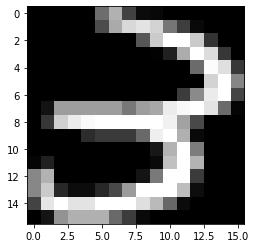
\includegraphics[width=0.6\textwidth]{Ans1_3_img.png} 
	        \captionsetup{labelformat=empty}
	        \caption{Fig: Gray scale image for three}
	        \label{fig:Gray scale image for three}



	        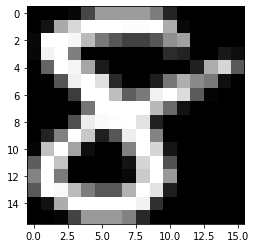
\includegraphics[width=0.6\textwidth]{Ans1_8_img.png} 
	        \captionsetup{labelformat=empty}
	        \caption{Fig: Gray scale image for eight}
	        \label{fig:Gray scale image for eight}

\end{figure}

\end{soln}

\clearpage


\item (5 pts) Putting the two data files together (threes first, eights next) to form a $n \times D$ matrix $X$ where $n=400$ digits and $D=256$ pixels.  Note we use $n\times D$ size for $X$ instead of $D\times n$ to be consistent with the convention in linear regression.   The $i$th row of $X$ is $x_i^\top$, where $x_i \in \R^D$ is the $i$th image in the combined data set.
Compute the sample mean $y = {1\over n} \sum_{i=1}^n x_i$.
Visualize $y$ as a 16x16 gray scale image.


\begin{soln}
	
	\begin{figure}[h!]
	        \centering
	        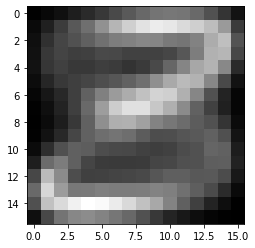
\includegraphics[width=0.6\textwidth]{Ans_2.png} 
	        \captionsetup{labelformat=empty}
	        \caption{Fig: Sample mean as Gray scale image}
	        \label{fig:Sample mean as Gray scale image}
	\end{figure}

\end{soln}


\item (10 pts) Center $X$ using $y$ above.  Then form the sample covariance matrix $S={X^\top X \over n-1}$.
Show the 5x5 submatrix $S(1\ldots 5, 1 \ldots 5)$.

\begin{soln} \\
$$S(1\ldots 5, 1 \ldots 5)=\\
\begin{bmatrix}
59.16729323  & 142.14943609  & 28.68201754 & -7.17857143 & -14.3358396 \\
142.14943609 & 878.93879073  & 374.13731203 &  24.12778195 & -87.12781955 \\
28.68201754 & 374.13731203  & 1082.9058584  & 555.2268797  &  33.72431078 \\
-7.17857143  & 24.12778195  & 555.2268797 & 1181.24408521 & 777.77192982 \\
-14.3358396  & -87.12781955  & 33.72431078 & 777.77192982 & 1429.95989975
\end{bmatrix}
$$
\end{soln}


\item (10 pts) Use appropriate software to compute the two largest eigenvalues $\lambda_1 \ge \lambda_2$ and the corresponding eigenvectors $v_1, v_2$ of $S$.
For example, in Matlab one can use eigs(S,2).  
Show the value of $\lambda_1, \lambda_2$.
Visualize $v_1, v_2$ as two 16x16 gray scale images.
Hint: their elements will not be in [0, 255], but you can shift and scale them appropriately.  It is best if you can show an accompany ``colorbar'' that maps gray scale to values. 

\begin{soln}
$$ \lambda_1 = 237155.24629049 $$
$$ \lambda_2 = 145188.35268683 $$

\begin{figure}[H]
	        \centering
	        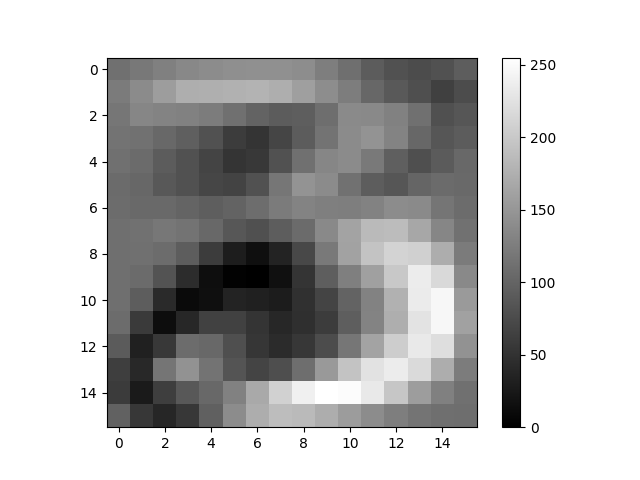
\includegraphics[width=0.5\textwidth]{4V1.png}
	        \captionsetup{labelformat=empty}
	        \caption{Fig: Eigen vector v1}
	        \label{fig:Eigen vector v1}
\end{figure}

\begin{figure}[H]
	        \centering
	        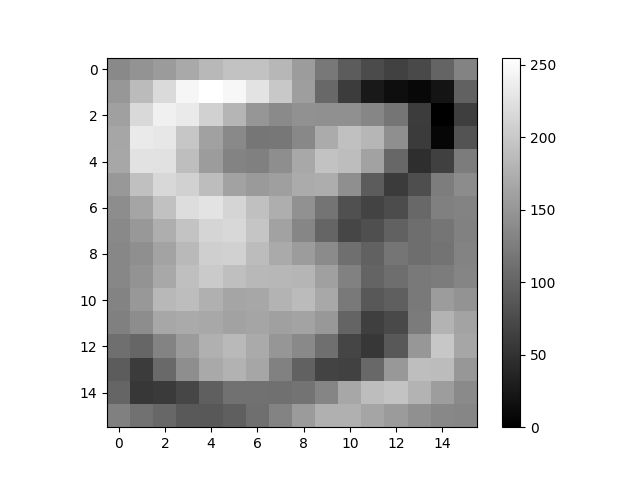
\includegraphics[width=0.5\textwidth]{4V2.png}
	        \captionsetup{labelformat=empty}
	        \caption{Fig: Eigen vector v2}
	        \label{fig:Eigen vector v2}
\end{figure}
\end{soln}



\item (5 pts) Now we project (the centered) $X$ down to the two PCA directions.   Let $V=[v_1 v_2]$ be the $D\times 2$ matrix.  The projection is simply $XV$.
Show the resulting two coordinates for the first line in three.txt and the first line in eight.txt, respectively.

\begin{soln}\\
Projection for first line in three.txt:
$[ 136.20872784, -242.62848028]$

Projection for first line in eight.txt:
$[-312.68702792,   649.57346086]$
\end{soln}




\item (5 pts) Now plot the 2D point cloud of the 400 digits after projection.
For visual interest, color points in three.txt red and points in eight.txt blue.
But keep in mind that PCA is an unsupervised learning method and it does not know such class labels.

\begin{soln} 

\begin{figure}[H]
	        \centering
	        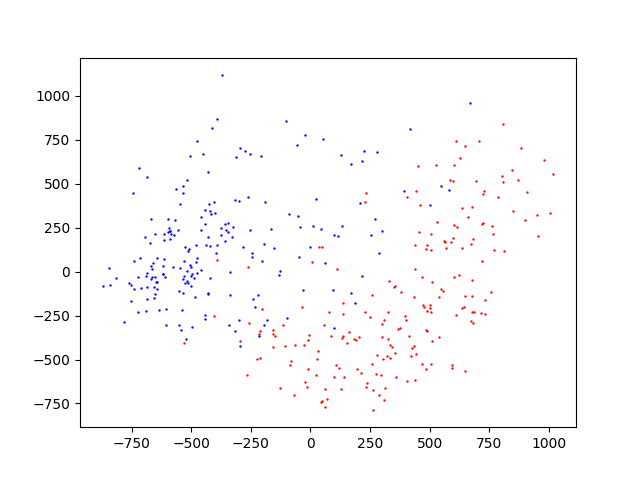
\includegraphics[width=0.7\textwidth]{Q6_YKWV.png}
	        \captionsetup{labelformat=empty}
	        \caption{Fig: 2D point cloud of the projected points}
	        \label{fig:2D point cloud of the projected points}
\end{figure}
\end{soln}

\end{enumerate}

\end{document}
